\documentclass{article}
\usepackage[utf8]{inputenc}% encodage du fichier source
\usepackage[francais]{babel}% rajouter éventuellement english, greek, etc.
\usepackage{listings}
\usepackage{hyperref}
\usepackage[margin=2.5cm]{geometry}
\usepackage{graphicx}
\hypersetup{urlcolor=,linkcolor=} % Does not apply color to href's
\lstset{
	tabsize=4,
	language=Java,
        basicstyle=\scriptsize,
        columns=fixed,
        extendedchars=true,
        breaklines=true,
		frame=single,
        showtabs=false,
        showspaces=false,
        showstringspaces=false,
        identifierstyle=\ttfamily,
        keywordstyle=\color[rgb]{0,0,1},
        commentstyle=\color[rgb]{0.133,0.545,0.133},
        stringstyle=\color[rgb]{0.627,0.126,0.941},
        numbers=left, 
        numberstyle=\tiny,
        xleftmargin=\parindent
}


\title{Android - TP2}
\date{Source, pdf et corrigé de ce TP
:\\ \href{http://tiny.cc/techmob}{http://tiny.cc/techmob}}

\begin{document}
\maketitle
L'objectif de ce TP est de réaliser une todo list (liste de choses à faire).\\
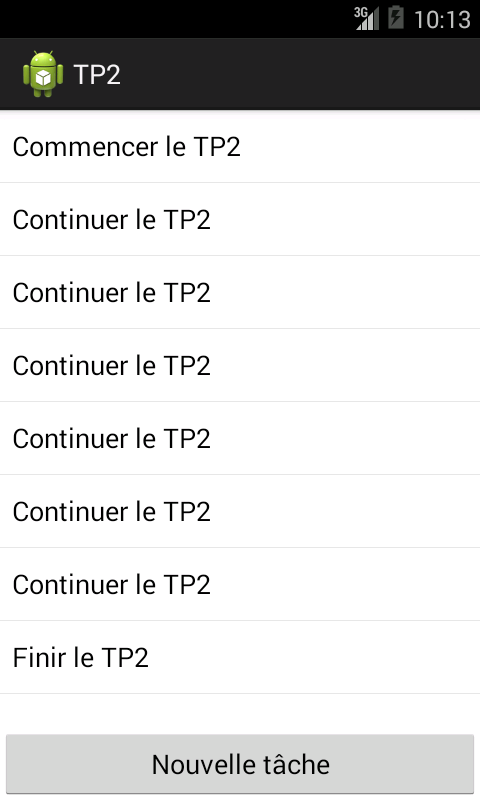
\includegraphics[width=100pt]{img/tp2screen1.png}
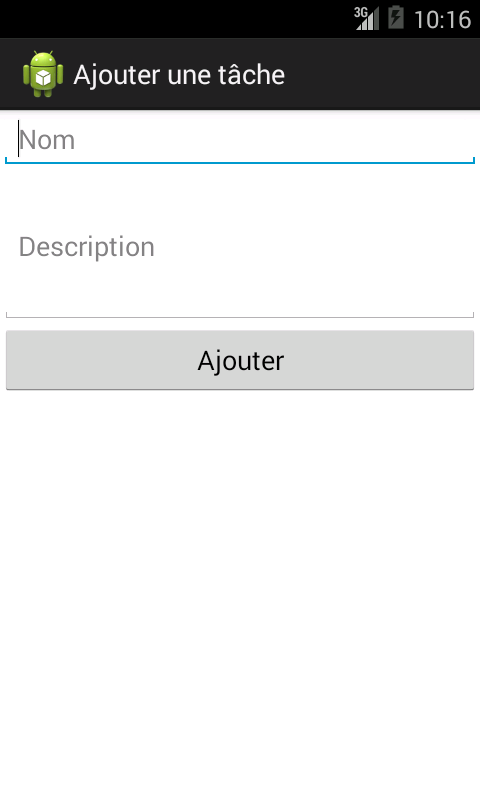
\includegraphics[width=100pt]{img/tp2screen2.png}
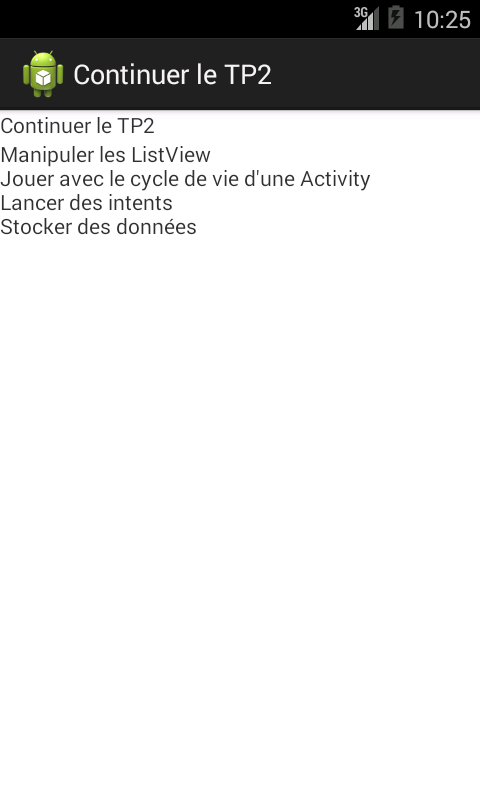
\includegraphics[width=100pt]{img/tp2screen3.png}\\
Ce TP fera appel aux notions suivantes :
\begin{itemize}
  \item ListView
  \item Listeners
  \item Cycle de vie de l'activity
  \item Intents
  \item Stockage de données
\end{itemize}
Il est fortement conseillé d'avoir le cours à portée de main et à ne pas hésiter
à se référer à la documentation officielle
\href{http://d.android.com}{http://d.android.com} ainsi qu'à la multitude de
tutoriaux disponibles.
\section{L'écran principal : affichage des tâches}
\begin{itemize}
  \item Créer un nouveau projet android avec les mêmes paramètres que dans le
  TP1 (EmptyActivity et Android 4.4 comme API min, max, cible)
  \item Modifier le layout de cette activity pour y placer une ListView qui
  prendra toute la largeur et toute la hauteur
\end{itemize}
\begin{enumerate}
 \setcounter{enumi}{0}
 \item Quel composant est chargé de faire le lien entre les données et la
 ListView ? (on l'implémentera plus tard)
 \end{enumerate}
 On souhaite ajouter un bouton ``ajouter une tâche'' en dessous de la ListView.
 \begin{enumerate}
 \setcounter{enumi}{1}
\item Pourquoi un LinearLayout ``naïf'' ne convient t'il pas ?
\end{enumerate}
\begin{itemize}
 \item En utilisant un RelativeLayout, placer le bouton en bas de l'écran
  \item Obtenir le même résultat en utilisant la propriété layout\_weight de
  LinearLayout au lieu du RelativeLayout
  \item Ecouter les clicks sur le bouton et afficher un Toast à chaque click
\end{itemize}
\section{Un écran secondaire : ajout d'une tâche}
\begin{itemize}
  \item Créer une deuxième activity
  \item Ajouter deux champs de texte modifiables (nom et commentaires) ainsi
  qu'un bouton ``ajouter'' à cette activity
\end{itemize}
\section{Enchainement des écrans}
\subsection{Dans un sens \ldots}
\begin{enumerate}
 \setcounter{enumi}{2}
\item On veut lancer l'activity d'ajout d'une tâche lors d'un click sur le
bouton ``ajouter une tache'' de l'activity principale.
Quel concept android va-t-on utiliser ?
\item Dans ce cas, est-il implicite ou explicite ?
\item Pensez vous qu'il faille passer des données lors de l'appel à l'activity ``ajouter une tâche'' ? Si oui, lesquelles ?
\end{enumerate}
\begin{itemize}
  \item Lancer l'activity d'ajout de tâche lors d'un click sur le bouton.
\end{itemize}
\subsection{\ldots et dans l'autre}

Lors d'un click sur le bouton ``ajouter'' de l'activity d'ajout, on souhaite retourner à l'écran principal.
 \begin{enumerate}
 \setcounter{enumi}{5}
\item Est-il judicieux de lancer un intent vers l'activity principale ? 
\end{enumerate}
 En réalité, android construit une pile des activités lancées (stack). \href{http://developer.android.com/guide/components/tasks-and-back-stack.html}{Documentation officielle sur le stack} 
  \begin{itemize}
  \item En faire l'éxpérience en allant sur l'activity d'ajout puis en appuyant
  sur le bouton retour de l'appareil.
  \item Utiliser la méthode
  \href{http://developer.android.com/reference/android/app/Activity.html#finish()}{finish()} de Activity pour fermer l'activity et ainsi revenir à l'écran principal lors d'un click sur le bouton ajouter.
 \end{itemize}
 
 \section{Place aux données !}
 \begin{itemize}
  \item Créer une classe métier déstinée à contenir les données : Element.
  Chaque élément de la todo list contiendra au moins un nom et une description.
 \end{itemize}
 \subsection{Afficher les données dans la ListView}
 \begin{itemize}
  \item Dans onCreate, créer un ArrayAdapter utilisant pour chaque
  view le layout \\android.R.layout.simple\_list\_item\_1
  \item Ouvrir le fichier XML de ce layout à l'aide de CTRL+click et constater
  sa simplicité
  \item Initialiser cet adapter avec une liste de Element générés à la volée
  \item Affecter cet adapter à la ListView
  \item Optionnel : compléter l'affichage de chaque élément en surchageant la
  méthode getView
 \end{itemize}
  \subsection{Stocker les données}
  \begin{enumerate}
 \setcounter{enumi}{6}
\item Quelle solution de stockage des données vous parait la plus adaptée ?
\end{enumerate}
On va opter ici pour une base de données SQLite
 \begin{itemize}
  \item Etendre la classe SQLiteOpenHelper pour mettre en place la base
  \item La base contiendra une unique table elements
  \item Lors de la création de la base, insérer quelques éléments dans la table
  \item Dans la méthode onCreate() de l'activity principale, remplir la ListView
  à partir des données contenues dans la base.
 \end{itemize}
 \subsection{Remplir les données}
 \begin{itemize}
  \item Lors d'un click sur le bouton ``ajouter'' de l'activity d'ajout, créer
  une instance d'Element et l'insérer en base.
 \end{itemize}
  \begin{enumerate}
 \setcounter{enumi}{7}
\item Pourquoi la ListView n'est elle pas mise à jour lors du retour sur l'activity principale ?
\end{enumerate}
 \begin{itemize}
  \item Utiliser le cycle de vie des activities pour recharger les données de la ListView lors du retour sur l'activity principale.
 \end{itemize}
 \section{Voir le détail d'un élément}
 \begin{itemize}
  \item Créer une activity de visualisation d'élement avec les champs utiles
  (nom, description \ldots)
  \item Ecouter les clicks sur les éléments de la ListView
  \item Lancer l'activity de visualisation lors d'un click sur un item de la liste
  \item Transmettre à l'activity le nom de l'item choisi
  \item Récupérer les données dans l'activity de visualisation et afficher les
  données de l'élément
 \end{itemize}
 \section{Pour aller plus loin}
	Wow, déjà tout fait ? Voici quelques pistes d'améliorations :
  \begin{itemize}
  \item Ajouter, sur l'activity principale, un bouton ``Exporter les données''
  qui génère un fichier contenant les élements. Proposer à l'utilisateur
  de partager ce fichier.
  \item Les données associées aux items sont pour l'instant minimales, pourquoi ne pas ajouter un identifiant, une date d'ajout, un statut (en cours, fait \ldots), une priorité, une catégorie \ldots ?
\end{itemize}
\end{document}


